\chapter{绪论}

北京时间2019年4月10日21时,人类首张黑洞照片在全球六地的事件视界望远镜(Event Horizon Telescope, EHT)发布会上同步发布。长久以来在电脑上模拟得到的黑洞影像,第一次真实地呈现在人们的面前,如图\ref{intro_black_hole}所示,该黑洞位于M87星系中心,质量为65亿倍的太阳质量,距离地球5300万光年。如此遥远的距离,科学家们采用了VLBI(very long baseline interferometry)技术来对黑洞进行观测成像。利用该技术,多个望远镜可以等效成一个孔径更大的望远镜,所能达到的角分辨率也就越高。为了对M87星系中心的黑洞进行成像,科学家们利用了全球多地8个亚毫米射电望远镜对黑洞进行了观测,它们北至西班牙,南至南极,观测得到了海量的数据。2017年时数据量就已经达到了10~PB(1~PB~=~1024~TB),2018年又增加了格陵兰岛望远镜,数据量继续疯狂增加。面对如此庞大的数据量,目前每个望远镜基地需要将观测得到的数据存入硬盘,然后将硬盘运送到VLBI数据中心进行处理,使得观测结果往往会滞后许多时间。光通信技术可以为如此巨量的数据传输提供支持。中国科学院VLBI系统,目前由上海,北京,昆明和乌鲁木齐等地的观测站和上海天文台VLBI数据中心组成,依托CNGI(China next generation internet),利用高速通信网络,将各观测站的观测数据,实时传输到上海数据中心,取代了传统的磁盘运输,可以将获得测量结果的最短滞后时间从若干天缩短到1分钟以内。

\begin{figure}[htb]
	\centering
	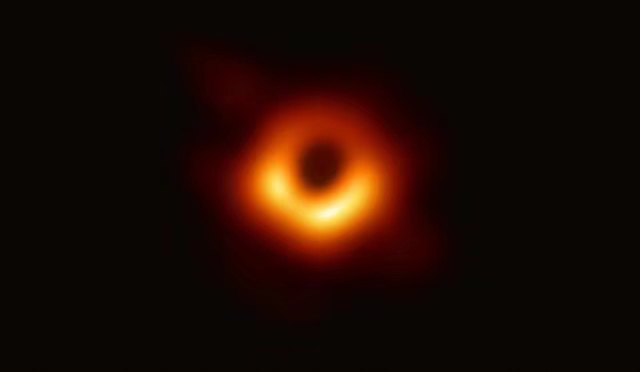
\includegraphics[width=13cm]{./Pictures/intro_black_hole.jpg}
	\captionsetup{justification=centering}
	\caption{人类首张黑洞照片}
	\label{intro_black_hole}
\end{figure}

光通信技术正是CNGI的主干网基础,它不仅可以提供长距离的大带宽数据传输服务,随着大数据时代的到来,数据中心需要存储海量的数据,并且各个机柜之间以及芯片与芯片之间需要进行大量的数据传输,在不远的将来,光互联技术将迈向最后一步进入到处理器内部进行数据的传输与处理。图\ref{intro_siliconphotonics}展示了电互联、硅基光通信和光纤通信在不同工作距离下的适用范围。当数据的通信速率达到10~GBps以上时,利用金属的电互联技术将会因为损耗、串扰与功耗等问题没法正常工作。而利用光互联技术,可以实现大带宽、低功耗和低时延的数据传输。因此,在信息传输领域,光子器件具有无可替代的地位。

\begin{figure}[htb]
	\centering
	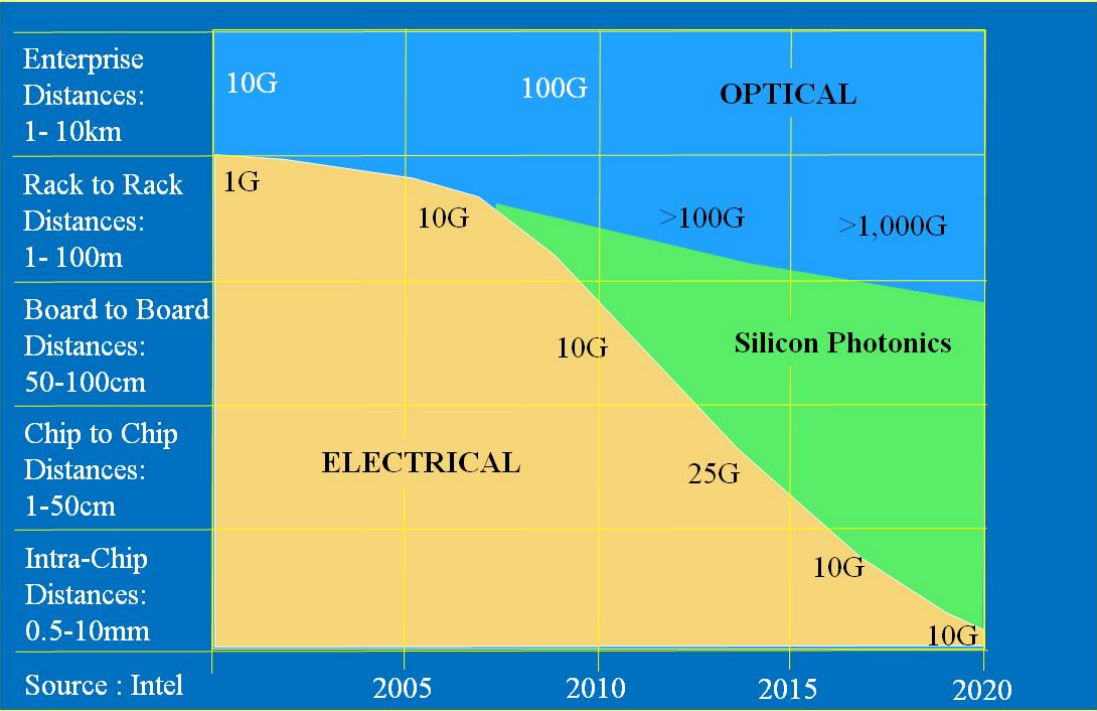
\includegraphics[width=13cm]{./Pictures/intro_siliconphotonics.png}
	\captionsetup{justification=centering}
	\caption{电互联、硅基光通信和光纤通信在不同通信距离下的适用范围\cite{zuffada2012industrialization}}
	\label{intro_siliconphotonics}
\end{figure}

传统光通信器件,由于价格高,尺寸大,功耗大已经无法满足芯片间以及芯片内部的应用,因此近几十年来,研究人员不断尝试新的材料平台,新的结构来实现大带宽、低功耗、低成本的解决方案。受到电子集成电路技术的启发,1969年,贝尔实验室的Stewart E. Miller提
出了集成光学的概念\cite{miller1969integrated},在片上集成激光器、调制器等光路系统代替组合式光路,利用器件的小型化可以避免热、机械、声等环境因素的影响,由此光互联技术进入了崭新的时代。

本章将首先简要介绍集成光学,然后介绍其中最有潜力的硅基光电子集成技术,接着着重讨论在硅基光电子集成技术中的一种重要光源---混合集成DFB激光器,最后介绍由作者制作的硅基混合集成自脉冲DFB激光器及其在三个领域的应用。


\section{集成光学简介}

集成光学的发展的动力首先来自于光通信的发展,作为信息载体,光子相比于电子具有独特的优势。例如,光子不带电荷,因而其传输过程中无电磁串扰的问题;光子具有频率、相位、振幅、偏振参数可以用于调制和检测,为通信提供了更多的可能性。

与传统的分立光学器件相比,集成光子器件的优势有:
\begin{enumerate}[(1)]
	\item 
	没有了传统光学器件的对准和光束准直问题,整个系统集成到同一块芯片上,稳定性更好;
	\item
	缩小了光学系统的体积,能够实现片上实验室(Lab on a Chip),提高了光学器件的密度,降低了总的功耗,使用也更加方便;
	\item 
	可以利用已经成熟的CMOS加工工艺,实现低成本、大规模的自动化生产。
\end{enumerate}

随着新材料的不断研发,集成光学所使用的材料也日益多样化,我们可以根据光波导所使用材料平台的不同,将集成光器件平台分为以下几种类型:

\begin{enumerate}[(1)]
	\item 
	掺杂型二氧化硅(SiO\SB{2})波导平台~~~~二氧化硅是最早被广泛采用的光波导材料之一,也是目前为止发展最成熟的无源器件平台。为了构成波导,至少要有两种折射率差的材料构成波导的芯层与包层,通常采用的办法是:在波导芯层中掺杂硼(P)、锗(Ge)等材料,使得其折射率比包层高大约1\%。由于折射率差比较小,故其波导尺寸较大,因此与早期的光通信中的光纤模式比较匹配,方便耦合,得到了广泛的应用。但也正是因为其波导尺寸比较大,不利于提高集成度,且二氧化硅属于无源材料,无法用其制作激光器、调制器、探测器等有源器件,也限制了其的应用。
	\item 
	聚合物波导平台~~~~聚合物材料是新近发展起来用于光电子器件领域的材料。该类波导的热光系数与电光系数都比较大,通过外场极化的方法可以获得高于LiNbO\SB{3}等无机晶体的电光系数,非常适合用于制作光开关与光调制器等器件。聚合物波导还具有材料配置方便、成本低廉等优点,只需要通过旋涂聚合物材料,曝光显影就能够制作,且工艺与半导体工艺相兼容,具有很好的发展前景。此外,几乎任何材料都可以作为聚合物的衬底,方便了聚合物与其他材料的集成。但是另一方面,聚合物材料容易老化,可靠性较差,这不利于提高器件的稳定性,且大部分聚合物无法承受较高的温度,不适用于CMOS工艺的大规模生产。
	\item 
	绝缘体上硅(silicon-on-insulator, SOI)波导平台~~~~绝缘体上硅材料是一种广泛用于制作集成电路的材料,利用现有的CMOS加工工艺,硅光集成芯片加工成本低,能够实现大规模生产。同时,硅材料具有优异的光学、电学和热学性能,硅材料在1.1~$\mu m$\~{}7~$\mu m$波段的光损耗很低,其氧化物SiO\SB{2}的折射率为1.46@1550 $nm$,与其本身折射率3.455@1550 $nm$相差很大,非常适合作为包层,能够对光形成很强的束缚,实现亚微米尺寸的波导。绝缘体上硅平台唯一不足的是,硅是一种间接带隙材料,无法实现高效率地发光,同时硅的电光效应较弱,故也无法制作高性能的电光调制器,由于其对通信波段的光没有吸收,故也无法制作探测器。研究人员们也找到了很多办法来解决绝缘体上硅平台的这些问题,比如通过混合集成的办法集成激光器与调制器\cite{ma2017demonstration,fang2006electrically},利用等离子体色散效应来实现速度达到10~Gbps以上的光调制器\cite{manipatruni2007high,fujikata201025,xiao201360}。
	\item 
	氮化硅(Si\SB{3}N\SB{4})波导平台~~~~氮化硅作为一种CMOS工艺中常用的掩模材料,近年来其优良的光学性能逐渐被人们发现并利用\cite{moss2013new}。氮化硅材料拥有比硅平台更低的损耗,以及较强的二阶非线性效应,因此在非线性研究领域受到了广泛的关注。氮化硅的低损耗窗口还包括可见光波段,且其有较高的折射率,故在可见光波段器件方面具有非常重要的应用。氮化硅还具有可调的色散特性,使其在光通信领域也有重要的应用。其缺点与绝缘体上硅平台类似,即也无法直接在其上制作有源器件,需要用混合集成技术才能实现。
	\item
	III-V族波导平台~~~~III-V族材料由于其直接带隙特性,通过调节不同元素的比例,其发光光谱可以从可见光一直到红外波段,能够满足照明、通信等方面的各种需求。III-V族材料可以实现光源、光放大器、调制器、探测器、波分复用器等器件,是作为光通信的理想材料。但是,由于III-V材料不易制做大尺寸的晶圆,加工成本较高,产品良率较低,使得其实现大规模商业化应用还有一定的困难。
	\item 
	铌酸锂(LiNbO\SB{3}波导平台~~~~LiNbO\SB{3}是一种比较成熟的多功能晶体,得益于其具有线性电光效应(Pockel effect, 普克尔效应),是制作电光调制器非常好的材料。LiNbO\SB{3}材料常通过掺杂来形成折射率差构成光波导,基于LiNbO\SB{3}的分立器件已经得到广泛应用。近年来,由于铌酸锂单晶薄膜的成功开发,其在集成领域的应用也开始崭露头角\cite{wang2018integrated,he2019high}。
\end{enumerate}

\begin{figure}[htb]
	\centering
	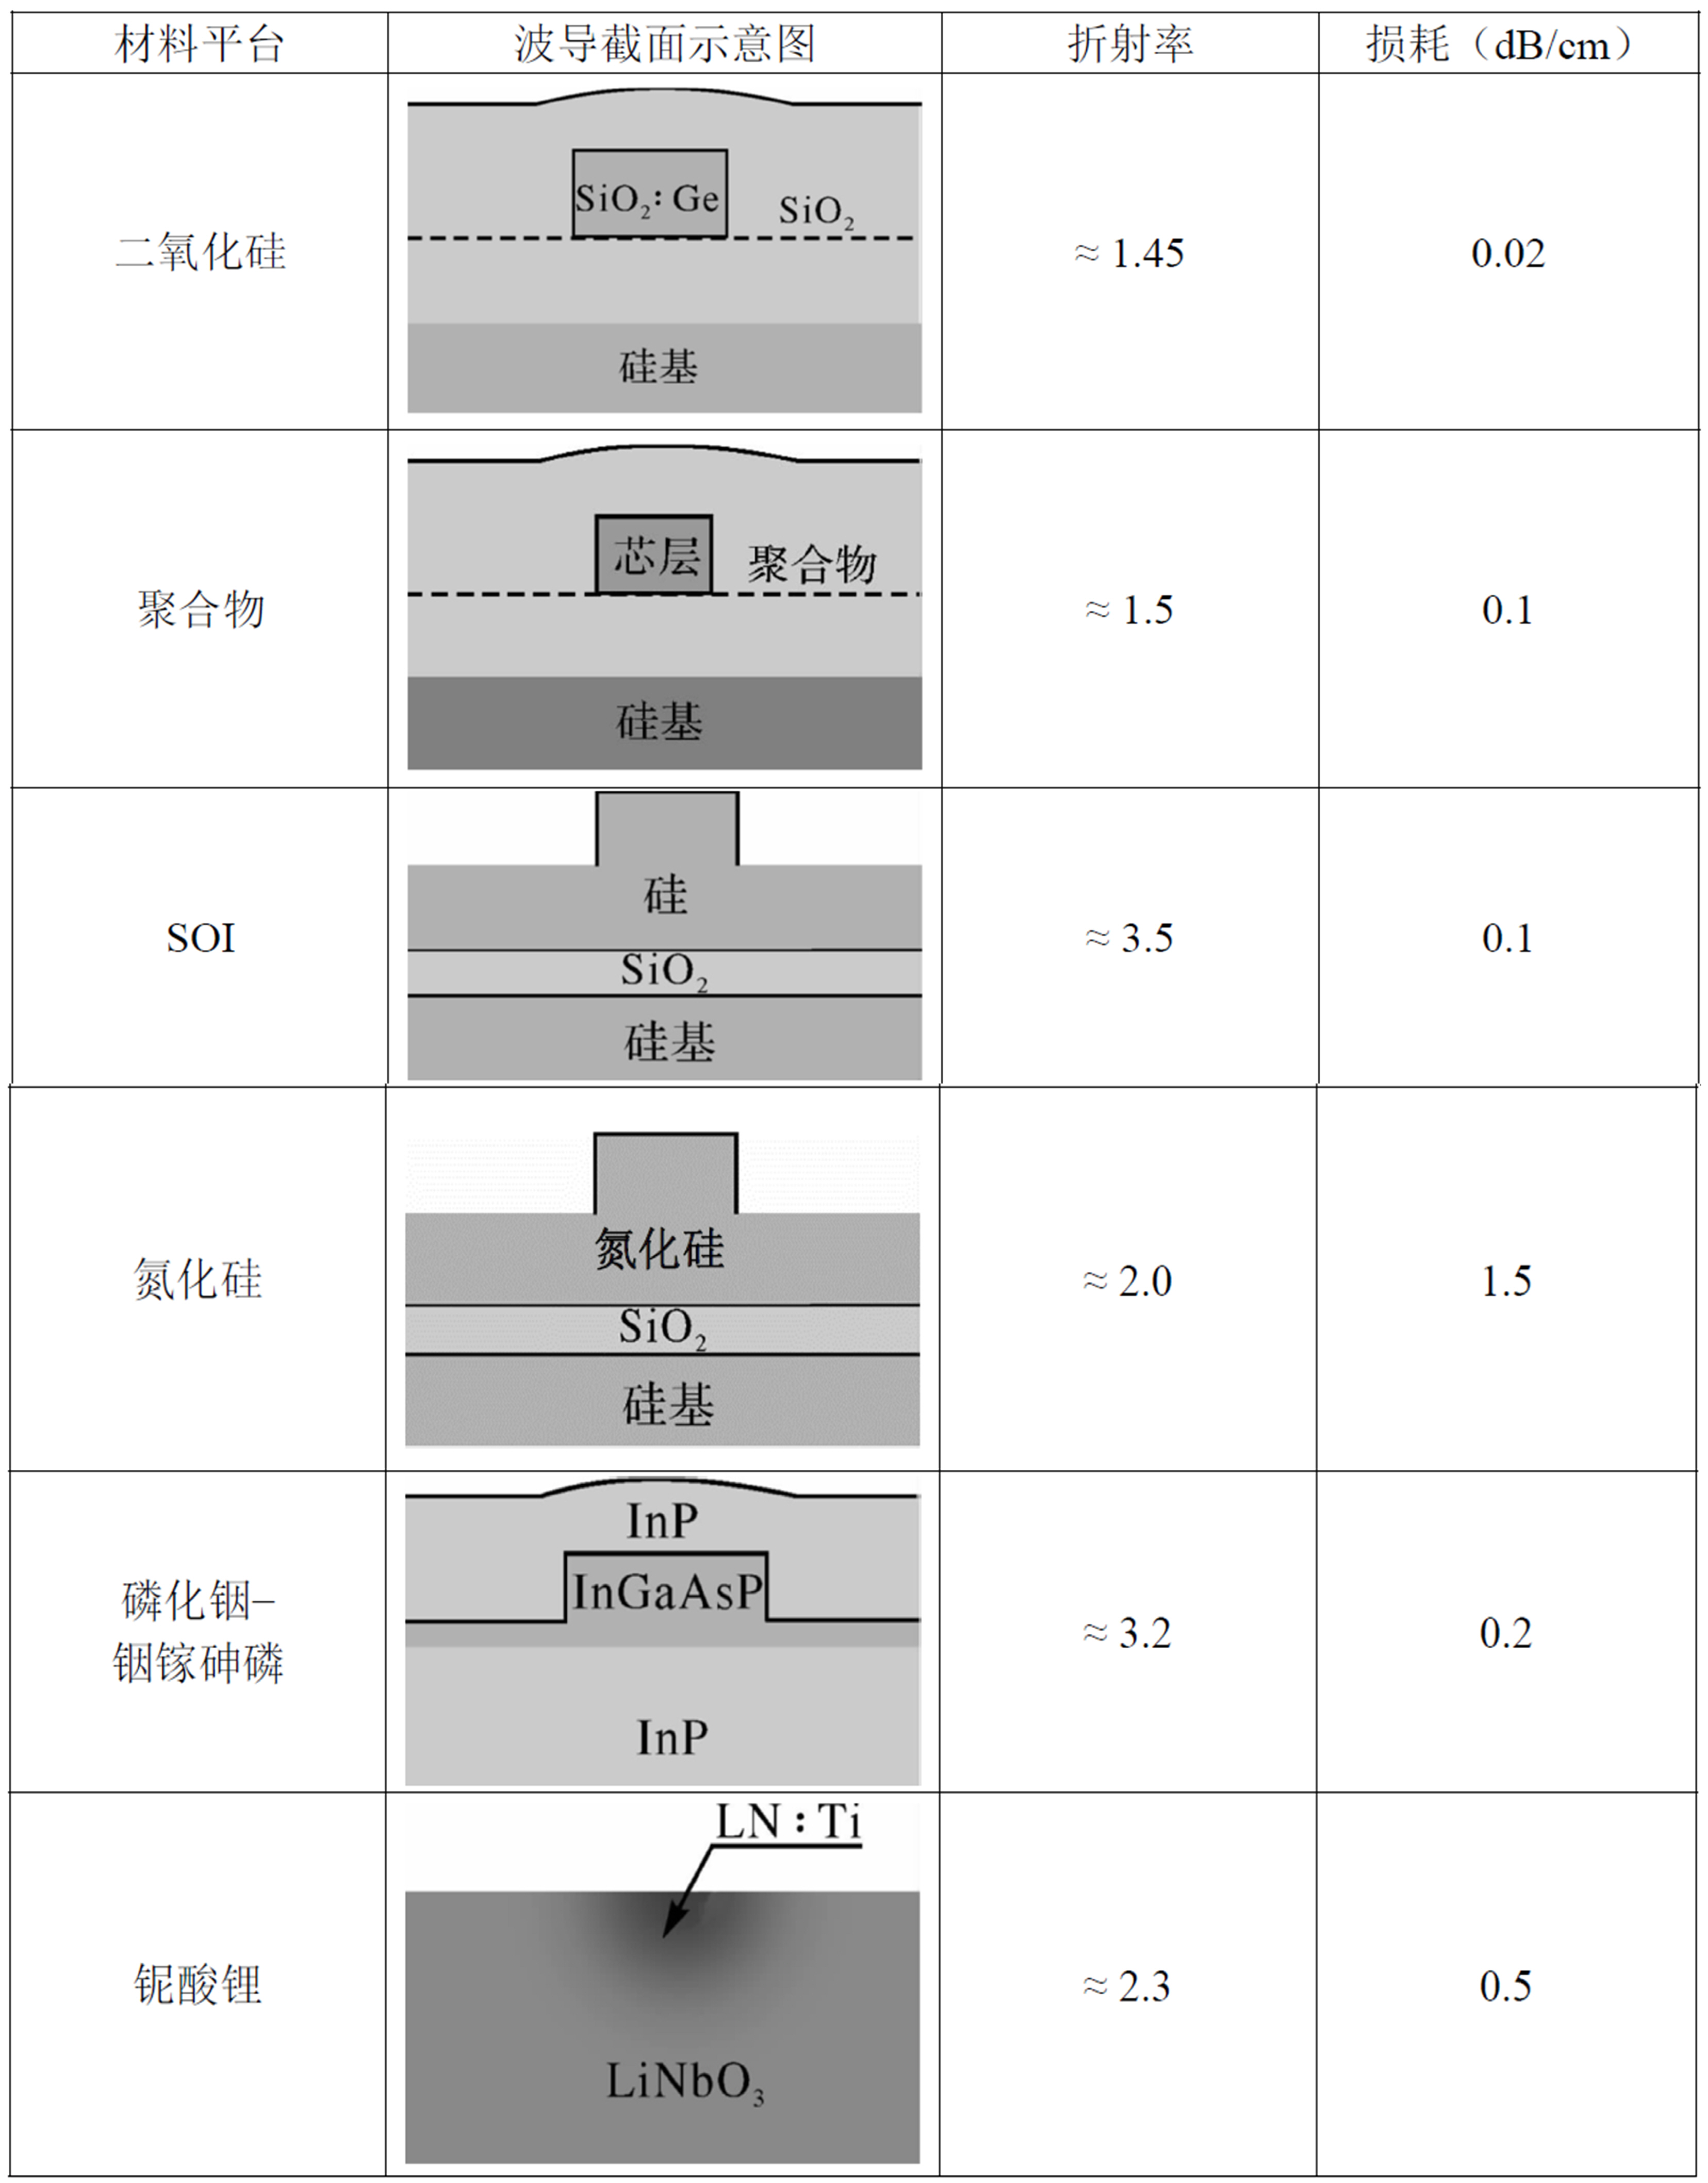
\includegraphics[width=13cm]{./Pictures/intro_materialplatform.jpg}
	\captionsetup{justification=centering}
	\caption{不同材料平台光波导平台\cite{hslwngzjc}}
	\label{intro_materialplatform}
\end{figure}

图\ref{intro_materialplatform}总给出了以上几种材料平台的波导结构以及其在通信波长λ@1550 $nm$的折射率和损耗。如上所述,各个平台都有相应的缺点与优点。在集成光学刚发展起来时,因为集成规模较小而更多的使用分立器件,往往根据器件的功能需求,选择最佳的平台以实现最佳的性能,比如,制作分立的激光器,往往利用III-V族材料平台,分立的调制器,往往采用铌酸锂(LiNbO\SB{3})波导平台。但是随着集成光学的发展,高密度的集成越来越受到关注,绝缘体上硅平台由于芯层与包层之间折射率差达到58\%,能够实现非常好的光限制,使得该平台成为高密度集成光学芯片的最好选择。

\section{硅基光电子集成技术}

硅基光子学最大的优势在于其制作工艺与当今非常成熟的CMOS(complementary metal-oxide semiconductor)工艺相兼容,且由于其特征尺寸远远大于晶体管的特征尺寸,故可以利用淘汰的CMOS生产线来制作硅基光电子器件,实现大规模自动化生产,制作成本大大降低,故硅基光子学已经被广泛认为是下一代通信技术的关键。

1985年,基于SOI平台的波导结构首次被研究并使人们意识到集成硅基光电子集成技术的潜力\cite{soref1985single,reed2005silicon}。不久之后的1989年,Bookham技术公司就开始将硅波导实现商业化。20世纪90年代,Bookham技术公司研发了最早的硅光集成器件芯片-硅光芯片与光纤结合的陀螺仪与压力传感器芯片\cite{rickman2014commercialization};随后,硅基光子学的产业化方向逐渐转向光通信中的波分复用器件(wavelength-division-multiplexing, WDM),因为利用波分复用技术,可以大大提升光纤的通信容量。随着基于硅波导的p-i-n调制器与锗硅探测器和调制器的实现\cite{liu2005tensile,feng2014micron},在通信领域采用硅基光子学变得越来越有希望。Luxtera、Mellanox和Acacia等公司已经成功开发了基于硅基集成技术的100~Gbps的光收发模块和相干收发模块,并朝着200~Gbps和400~Gbps迈进\cite{boeuf2015recent,feng2014micron,doerr2014single},国内的旭创科技、光迅科技、海信宽带等则已经可以提供400~Gbps的收发模块,这些收发模块将用于提升超级计算机、和电信通信领域等的性能。

\begin{figure}[htb]
	\centering
	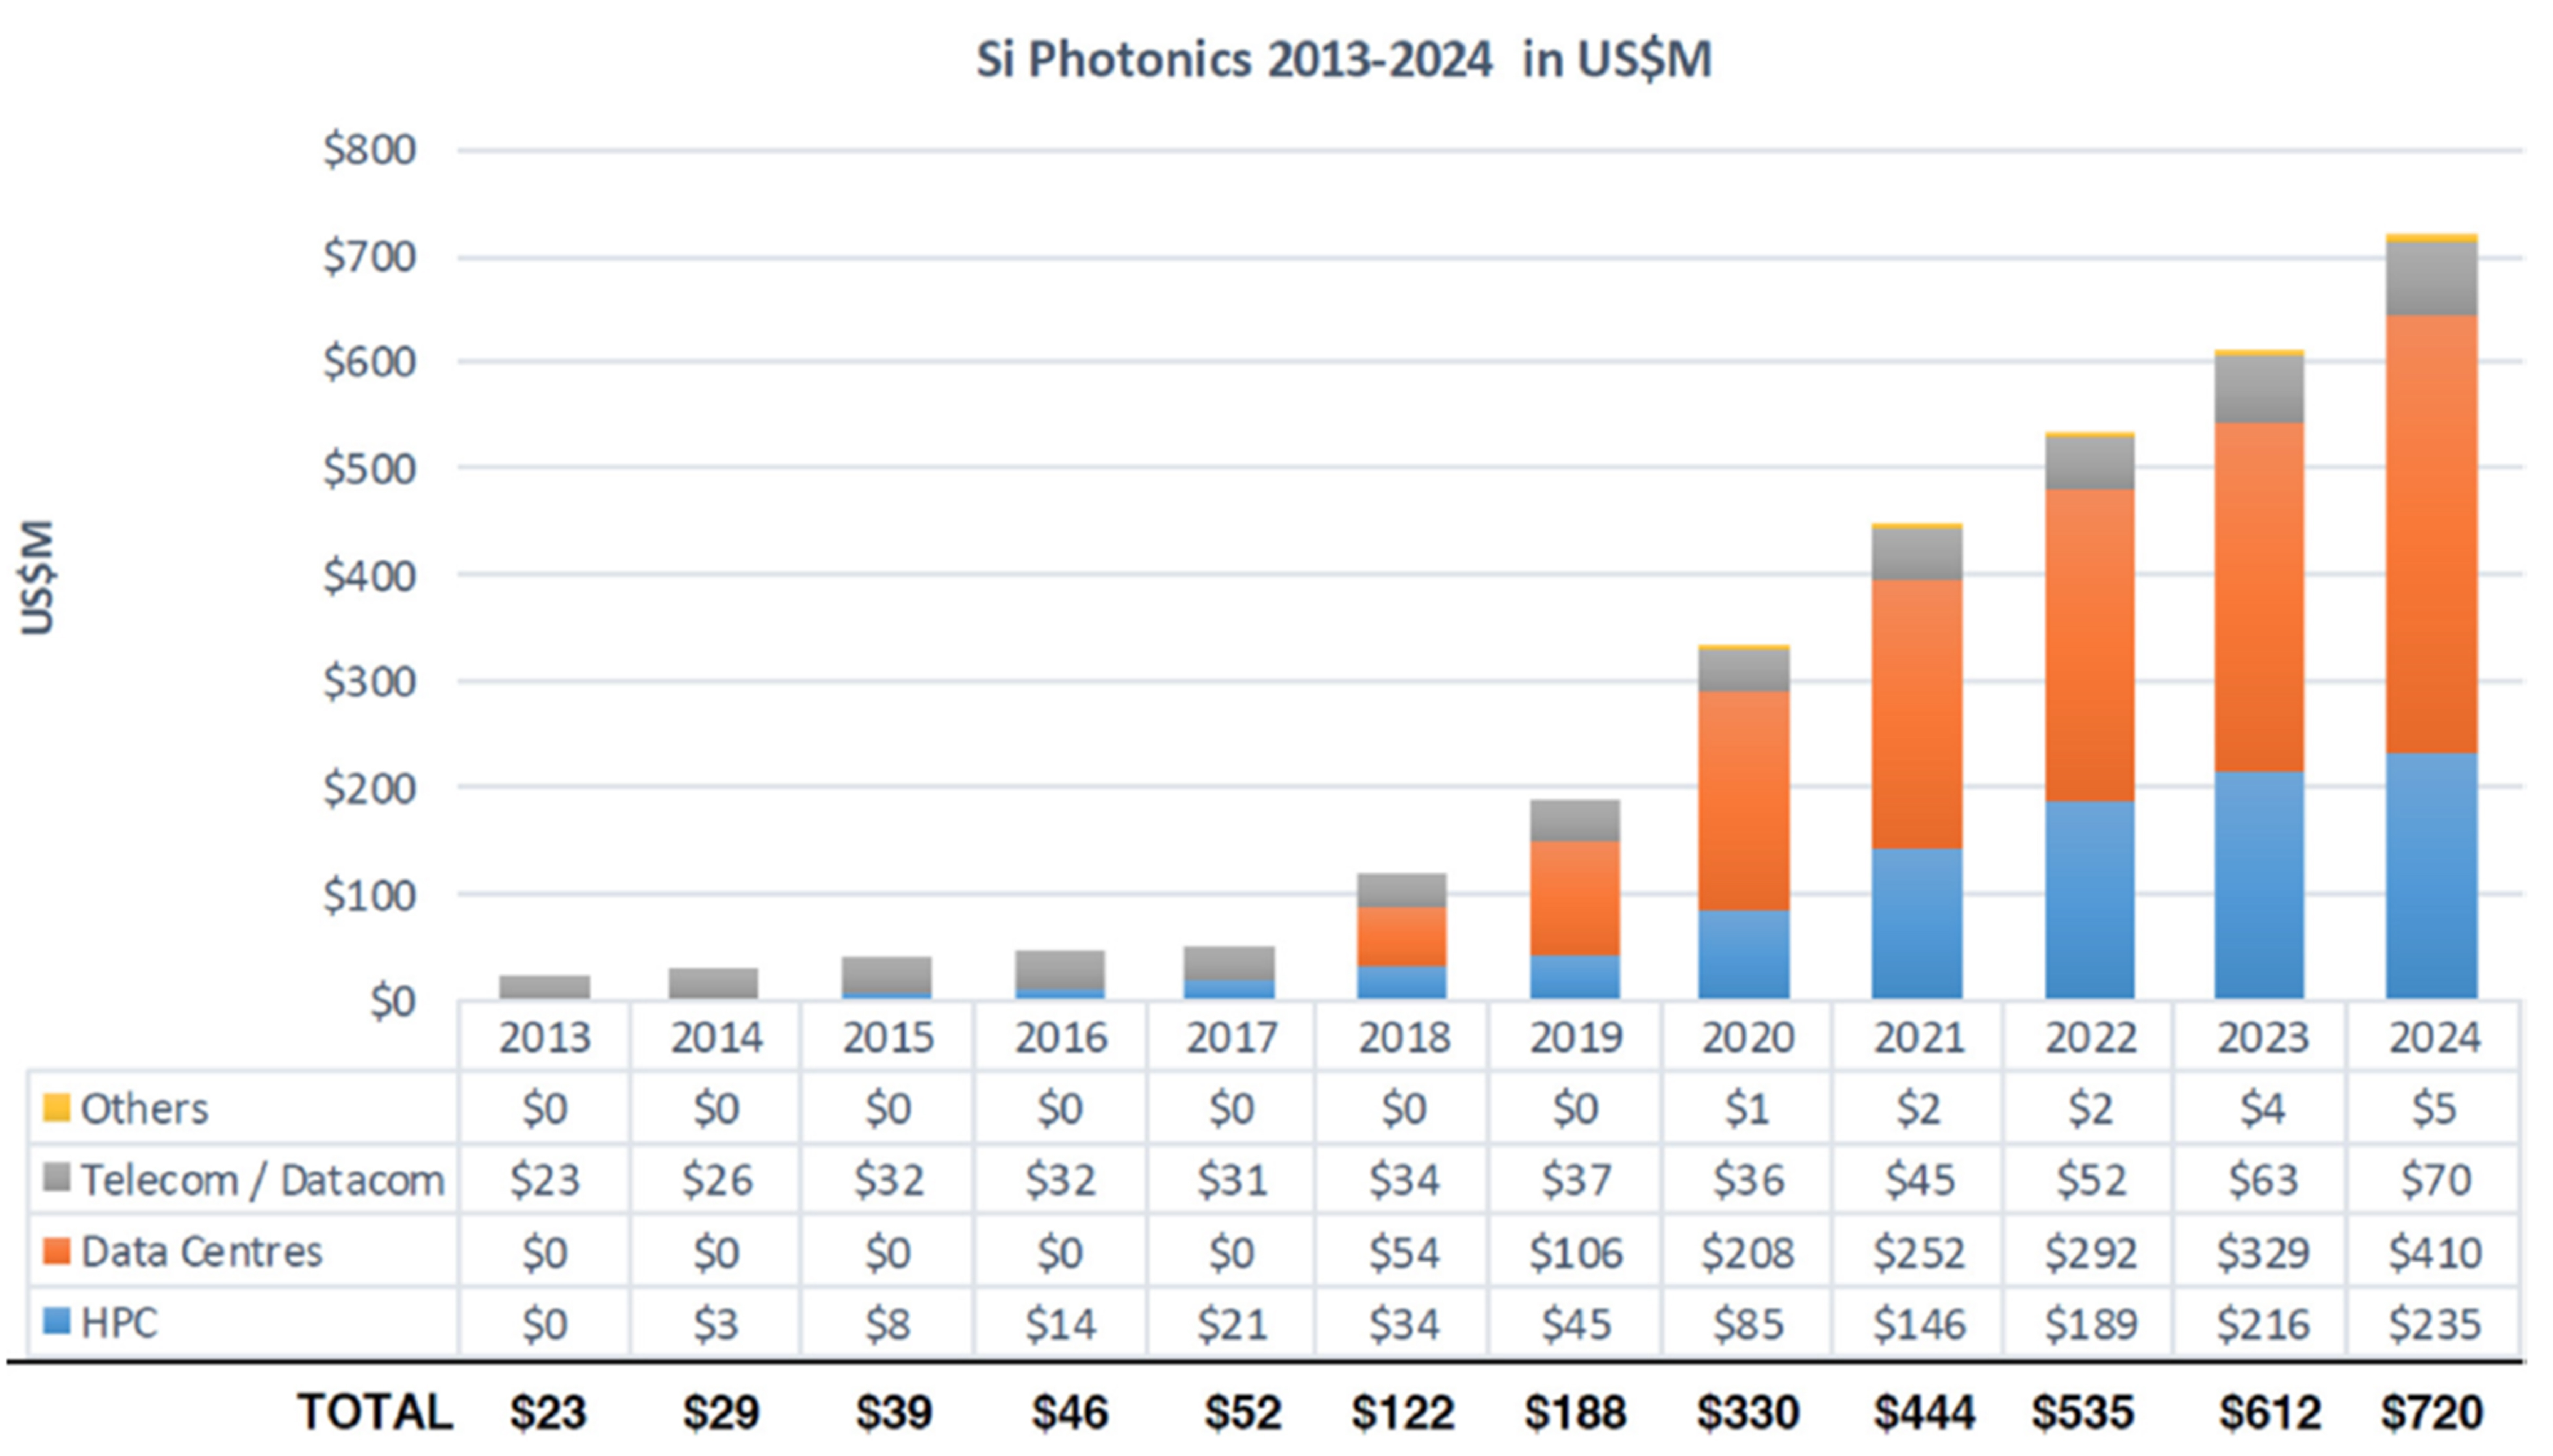
\includegraphics[width=14cm]{./Pictures/intro_siliconphotonicsmarket.jpg}
	\captionsetup{justification=centering}
	\caption{市场咨询机构Yole Développement对2013年至2024年硅光芯片市场的预测(来源:Silicon Photonics Report - Yole Développement; ‘Emerging optical data centers from big Internet companies (Googlem Facebook, ...) will be triggering the market growth in 2018...’ )}
	\label{intro_siliconphotonicsmarket}
\end{figure}

图\ref{intro_siliconphotonicsmarket}是市场咨询机构Yole Développement对2013年至2024年硅光芯片市场的统计与预测,2013年至2017年,硅光芯片主要用于电信和超级计算机行业,总体市场规模较小,2018年,硅光芯片将开始腾飞并且在未来会保持20\%以上的高速增长,主要得益于硅光芯片可以将数据传输的成本降低到\$1/Gbps,相比于之前的电互联和多模光纤互联成本更低,所以数据中心和超级计算机行业将会大规模部署。除了费用更低外,硅光芯片能耗也可以降低到pJ/bit量级,器件的稳定性也更好。

在典型的光互联系统中,最重要的组成部分就是光收发模块,其由发射机与接收机两部分组成,如图\ref{intro_transceiver}所示。在发射机中,经过CPU处理的数据通过调制器调制激光器的输出光,从而将所需要传输的数据加载到光波上。为了增加通信的容量,可以采用波分复用技术,将不同路的信号加载到不同波长的激光上。调制的方式可以采用直接调制或者外调制,直接调制是指通过调制激光器的驱动电流来调制激光器的输出光强,外调制则是通过外接调制器来对激光器的输出光强进行调制。直接调制的优点是简单方便,但是由于调制时会改变激光器的载流子浓度,会出现频率啁啾效应,调制速率受限。外调制虽然所需要用到的调制器结构较为复杂,但具有良好的调制性能,由其是在高速率的状态下。

\begin{figure}[htb]
	\centering
	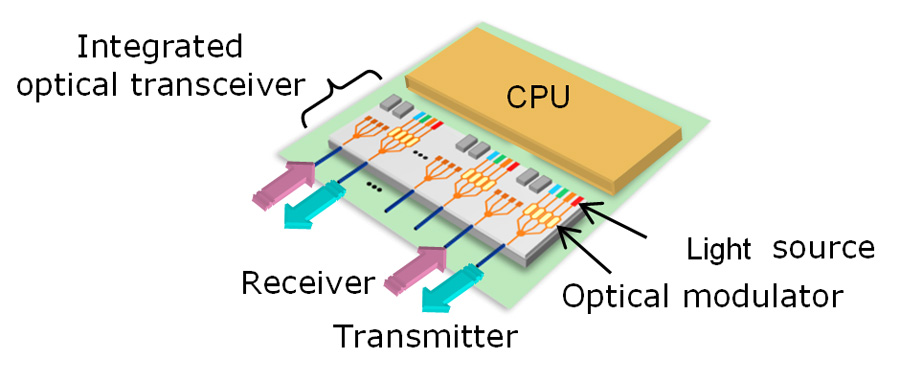
\includegraphics[width=14cm]{./Pictures/intro_transceiver.jpg}
	\captionsetup{justification=centering}
	\caption{光收发模块示意图(Fujitsu)}
	\label{intro_transceiver}
\end{figure}

无论是直接调制还是外调制,都需要有能够在片上集成的高效单模激光器,但是由于硅的间接带隙特性,其发光效率特别低,虽然研究人员已经利用拉曼效应(Raman scattering)和布里渊效应(Brillouin scattering)成功制作了硅基激光器\cite{otterstrom2018silicon,rong2007low},但该类激光器都需要采用光泵浦的方式,不适合大规模用于光互联通信系统中,要利用硅制作高效地电泵浦激光器仍然非常困难。

\begin{figure}[htb]
	\centering
	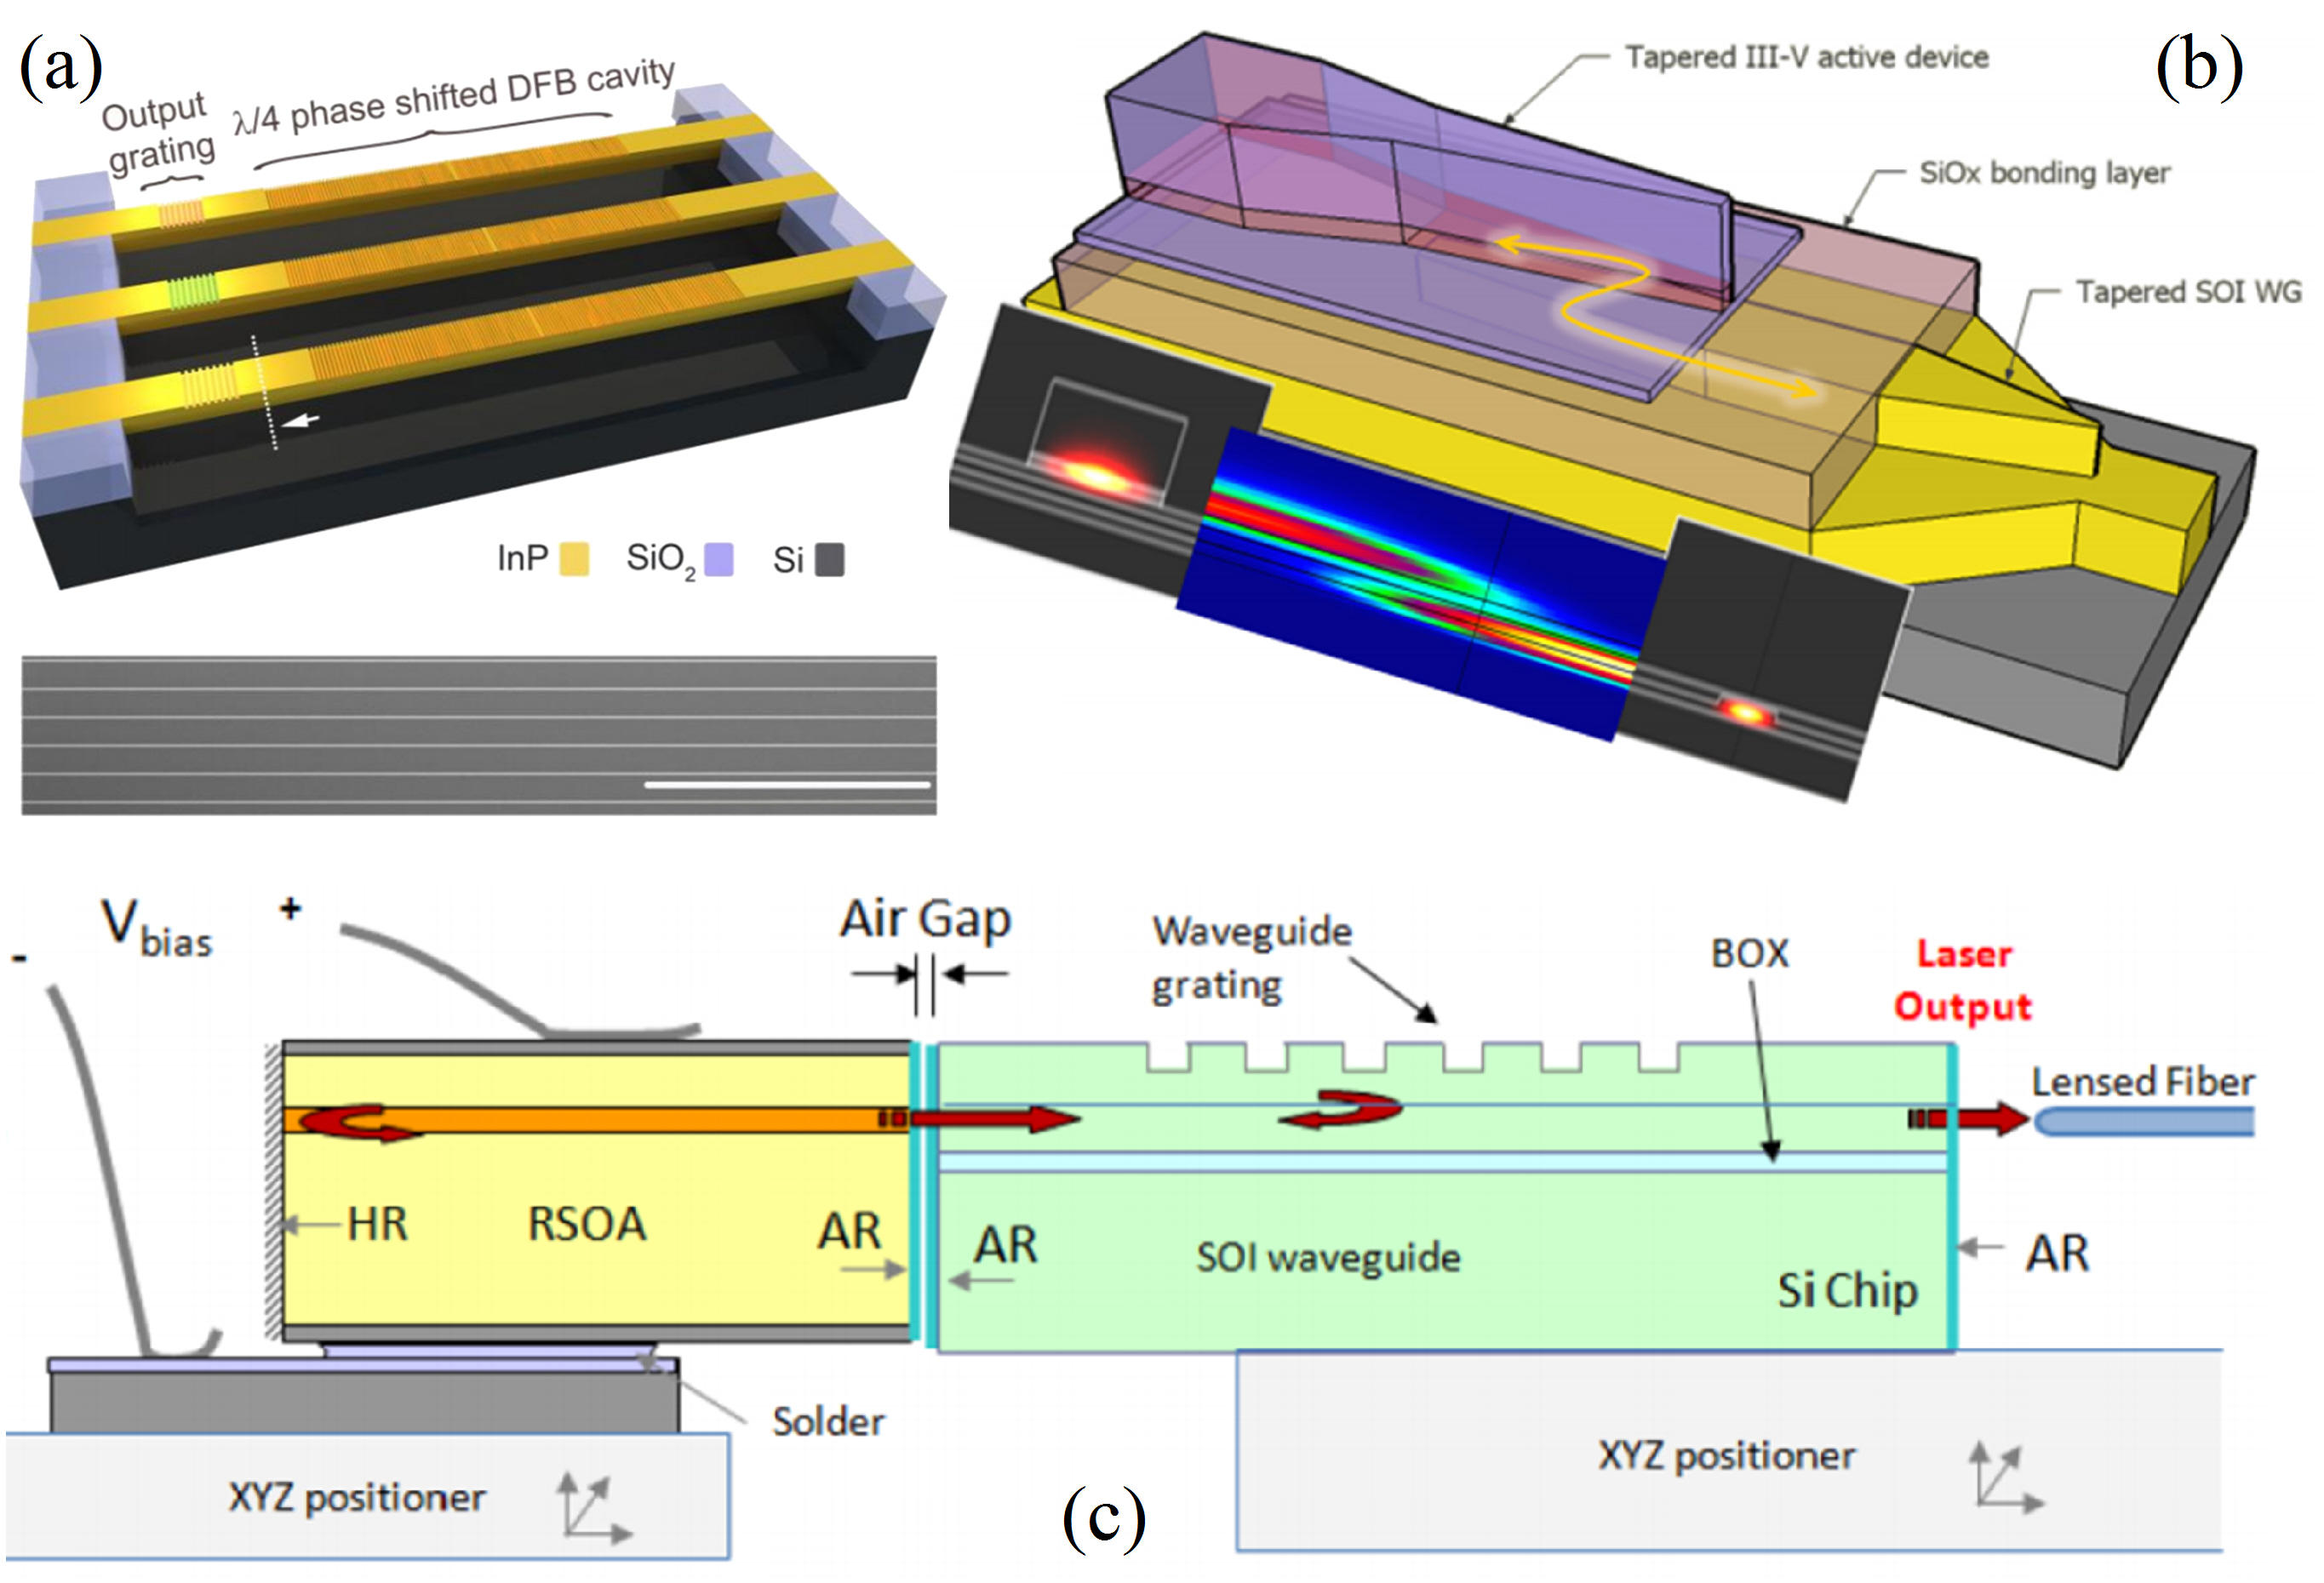
\includegraphics[width=14cm]{./Pictures/intro_lasers.jpg}
	\captionsetup{justification=centering}
	\caption{三种硅基集成激光器的方案:(a)在硅上外延生长IIII-V材料制作的激光器\cite{wang2015room};(b)~III-V材料与硅键合制作的激光器\cite{keyvaninia2013demonstration};(c)~III-V有源增益区与硅器件通过Flip-Chip键合制作的激光器\cite{zilkie2012power}}
	\label{intro_lasers}
\end{figure}

由于无法利用硅材料在片上实现高效的电泵浦激光器,人们想到了利用III-V族有源增益材料与硅结合的方法来制作硅上的光源\cite{heck2013hybrid,keyvaninia2013heterogeneously},一般有三种方式来实现硅与III-V族材料的集成\cite{bowers2014path}。第一种方法是直接在硅层上面生长III-V族外延层,由于硅与III-V族材料的晶格与热膨胀系数不匹配(Si与InP有8\%的晶格常数不匹配度,84\%的热膨胀系数不匹配度),通常会使用锗作为中间缓冲层来释放晶格不匹配造成的应力。图\ref{intro_lasers}(a)所示为Wang等人通过在硅波导上利用羟化四甲铵腐蚀液(TMAH)腐蚀出V型凹槽,通过选择性生长的方法,可以将因晶格不匹配产生的线位错与反相面限制在20~$nm$厚度内,故不会影响III-V族材料制作的激光器的性能\cite{wang2015room},但是该激光器还是需要光泵浦而不是电泵浦,因此不适用于片上大规模应用;第二种是利用键合的方法,将III-V晶片先键合到硅波导上,这一步不需要精确的对准,键合完之后在III-V晶片上制作激光器的结构,硅波导与III-V波导的光通过垂直耦合的方式进行耦合。图\ref{intro_lasers}(b)所示为Keyvaninia等人利用BCB作为键合层,将III-V族材料键合到SOI上提供增益,利用SOI上的腔结构提供反馈,制作的电泵浦激光器,在20~$^{\circ}$C条件下可以实现最大输出功率为10~$mW$\cite{keyvaninia2013demonstration};第三种是采用Flip-Chip的方法实现III-V族材料波导与硅波导的端面耦合,通过III-V族材料提供增益,硅波导上的谐振腔提供反馈,实现激光的输出。图\ref{intro_lasers}(c)所示为Zilkie等人利用半导体放大器(SOA)与硅波导DBR反射镜,通过Flip-Chip的方法实现端面耦合,制作的激光器最大输出功率为6~$mW$\cite{zilkie2012power}。

目前,考虑到直接外延生长III-V族材料制作的激光器由于缺陷的影响寿命比较短\cite{liu2015reliability,sun2016room},主要采用硅与III-V族材料键合的方式来制作片上激光器(heterogeneous integration)。这样可以充分利用两者的优势,III-V材料具有直接带隙材料的特点,可以提供较高的增益,而且能带间隔可以通过不同组分的含量进行调节,实现不同波长的激射;硅基光子平台可以在通讯波段提供低损耗的波导(<1~dB/$cm$),而且由于其超高的折射率差可以实现较小的波导弯曲,实现高密度的集成。目前,基于硅基光子平台的无源器件已经被大量的制作完成,包括阵列波导光栅(AWG),刻蚀衍射光栅(EDG),多模干涉器(MMI),微环谐振腔,耦合光栅等等\cite{asghari2011silicon,jalali2006silicon},可以实现片上光传输的种种功能。利用键合的方式将III-V材料与SOI混合集成,研究人员已经实现了在SOI上的电泵浦激光器,高速调制器、探测器和半导体光放大器\cite{liang2010hybrid,roelkens2010iii,liang2010recent,duan2014hybrid}。

在混合集成激光器中,DFB激光器(distributed feedback laser)由于其稳定的单模特性,工艺简单,性能优良而被广泛采用。

\section{硅基III-V混合集成DFB激光器}

DFB激光器也叫分布反馈式激光器,是一种在光收发模块中常用的端面出射激光器,与另一种常用的DBR激光器(distributed brag reflector laser)不同的是,其布拉格反射光栅位于激光器的腔内,如图\ref{intro_dfb_laser}所示。布拉格光栅可以位于包层作为折射率实部的调制,叫做折射率耦合;也可以位于增益材料中作为折射率虚部的调制,叫做增益耦合。它们在实际激光器制作过程中的区别是,是否需要$\Lambda/2$的相移来实现单模激射($\Lambda$为布拉格光栅的周期)。布拉格光栅的周期需要经过设计使其反射波长位于增益介质的增益带宽内,在光通信波段,常用的增益介质为基于InP的三元或者四元外延结构,如InGaAsP和InGaAlAs。

\begin{figure}[htb]
	\centering
	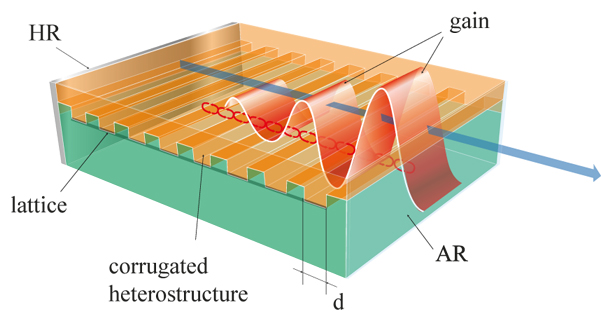
\includegraphics[width=11cm]{./Pictures/intro_dfb_laser.jpg}
	\captionsetup{justification=centering}
	\caption{DFB激光器示意图,AR: antireflection, HR: high reflection}
	\label{intro_dfb_laser}
\end{figure}

本文所研究的混合集成DFB激光器如图\ref{intro_heterogeneously_dfb_laser}所示,DFB光栅制作在SOI的硅上,光栅采用一阶光栅,以InGaAsP材料作为有源层的III-V芯片通过BCB键合到硅波导上,之后通过结合光刻与干法刻蚀或湿法刻蚀完成III-V波导的制作。硅波导与III-V波导之间的光通过反向锥形波导结构进行耦合,使得从有源区产生的激光通过硅波导上的耦合光栅输出,进行测试。通过控制BCB的厚度,可以控制光栅的耦合强度,从而提供了一种可以控制激光器性能的维度,比如可以通过增加BCB的厚度减少光在III-V波导中的比例来减小激光器的线宽\cite{yariv2016rethinking}。

\begin{figure}[htb]
	\centering
	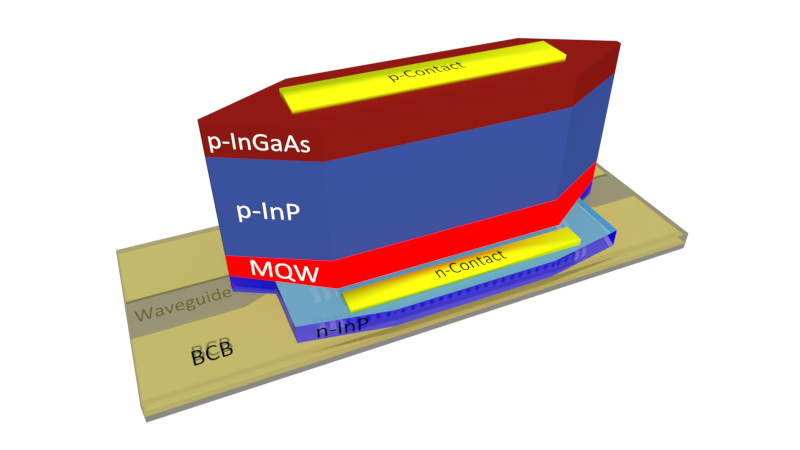
\includegraphics[width=15cm]{./Pictures/intro_heterogeneously_dfb_laser.png}
	\captionsetup{justification=centering}
	\caption{硅基III-V混合集成DFB激光器示意图}
	\label{intro_heterogeneously_dfb_laser}
\end{figure}

\section{DFB激光器的应用}

\subsection{微波光子领域的应用}

传统上微波信号是利用电子电路经过多级倍频来达到所需要的频率,然后通过同轴电缆进行传输,但是由于一些固有的和寄生的阻抗或者容抗限制,该种方法能够产生的微波信号频率与传输损耗都会受到限制,而且成本也较高。在过去三十多年来,微波光子学(microwave photonics, MWP)这门学科吸引了众多研究人员的注意,因为其可以将微波领域与光子学领域结合起来,实现在微波系统上实现起来特别复杂或者没法实现的功能。而且利用微波光子学,可以实现新的信息传输系统,实现微波信号的长距离低损耗传输\cite{capmany2007microwave,seeds2002microwave,seeds2006microwave,yao2009microwave}。其应用领域包括蜂窝天线,无线通信,卫星通信,有线电视,分布天线系统和医学成像等。

微波光子学最开始主要是利用分立的光电子器件和光纤来实现一些功能,比如微波信号的产生、分配、处理与分析,其器件昂贵笨重且不稳定,功耗也较大。随着硅基光电子集成技术的发展,微波光子学也开始朝着集成的方向发展,以实现低功耗与稳定的微波光子器件。

\begin{figure}[htb]
	\centering
	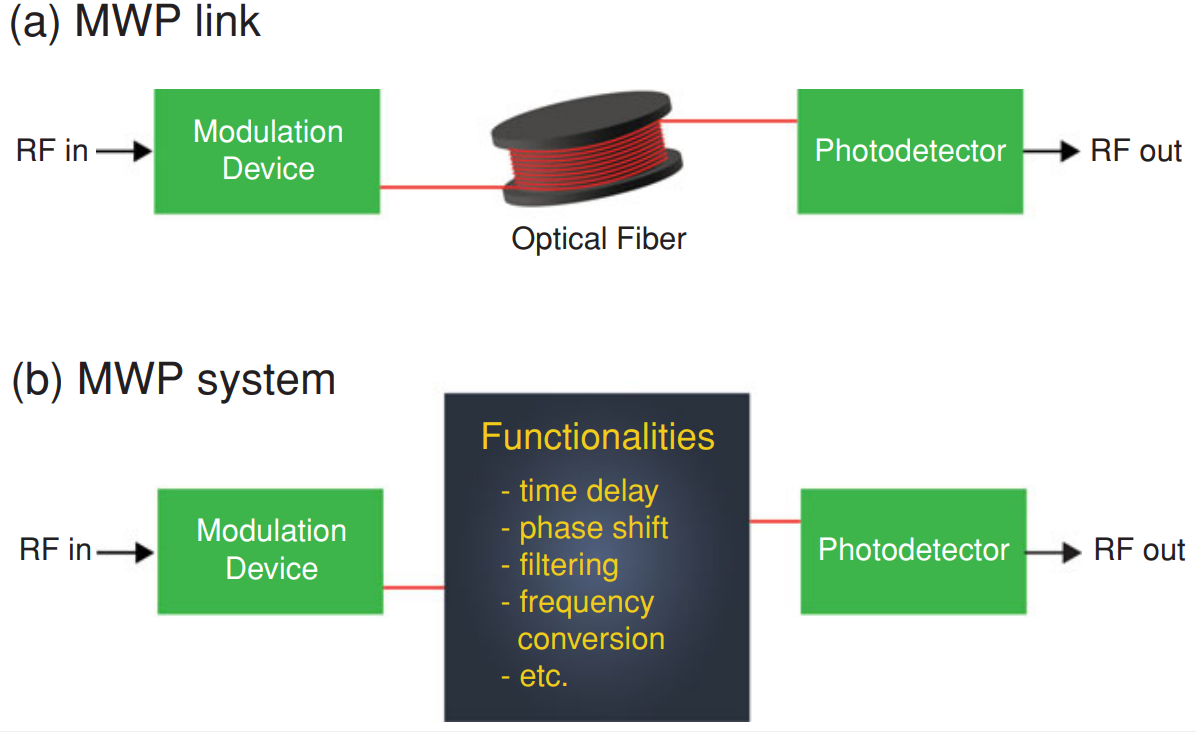
\includegraphics[width=14cm]{./Pictures/intro_mwp.png}
	\captionsetup{justification=centering}
	\caption{(a)典型的微波光子学链路示意图(b)简单的微波光子学系统组成示意图\cite{marpaung2013integrated}}
	\label{intro_mwp}
\end{figure}

图\ref{intro_mwp}(a)所示为典型的微波光子学链路示意图,微波信号经过调制器进行电光转换加载到光波上,经过光纤传输,然后探测器接收后光波之后将微波信号还原出来。图\ref{intro_mwp}(b)所示为典型的微波光子学系统示意图,微波信号经过调制器加载到光波上之后,可以在光频上进行时延,相移,滤波,频率转换等操作,然后再通过探测器转换到微波信号。利用光学方法进行处理可以实现更大的带宽,对不同的频率损耗均一,器件尺寸更小,不受电磁干扰影响,而且功耗也能够更低。

\subsection{光互联领域的应用}

外调制技术由于不会产生频率啁啾现象,可以减小光在光纤中传输的色散问题,使其对于需要经过光纤长距离传输的光通信系统来说相比于直接调制技术有明显的优势。但是对于短距离通信来说,直接调制相比于外调制有许多独特的优势。DFB激光器可以通过调制驱动电流大小来调制激光器的输出强度,这样一来,可以将光收发模块中的激光器与调制器融合成一个器件,可以降低系统的工艺复杂度,缩小总体器件的尺寸,还可以降低系统功耗。对于典型的马赫曾德外调制器,其往往需要较长的尺寸以换取较小的驱动电压,其尺寸往往达到数毫米。图\ref{intro_external_modulator}(a)所示为基于LiNbO\SB{3}的马赫曾德调制器,其长度为5~$mm$时,V$_{\pi}$为5.1~$V$,这对于调制速度要求不高但是对总体尺寸要求高的应用场景是不合适的。图\ref{intro_external_modulator}(b)所示基于III-V族材料的电吸收调制器,其插入损耗为5~dB,这意味着需要光源提供更高的功率来补偿调制器的损耗,从而导致整个系统的功耗增加。

\begin{figure}[htb]
	\centering
	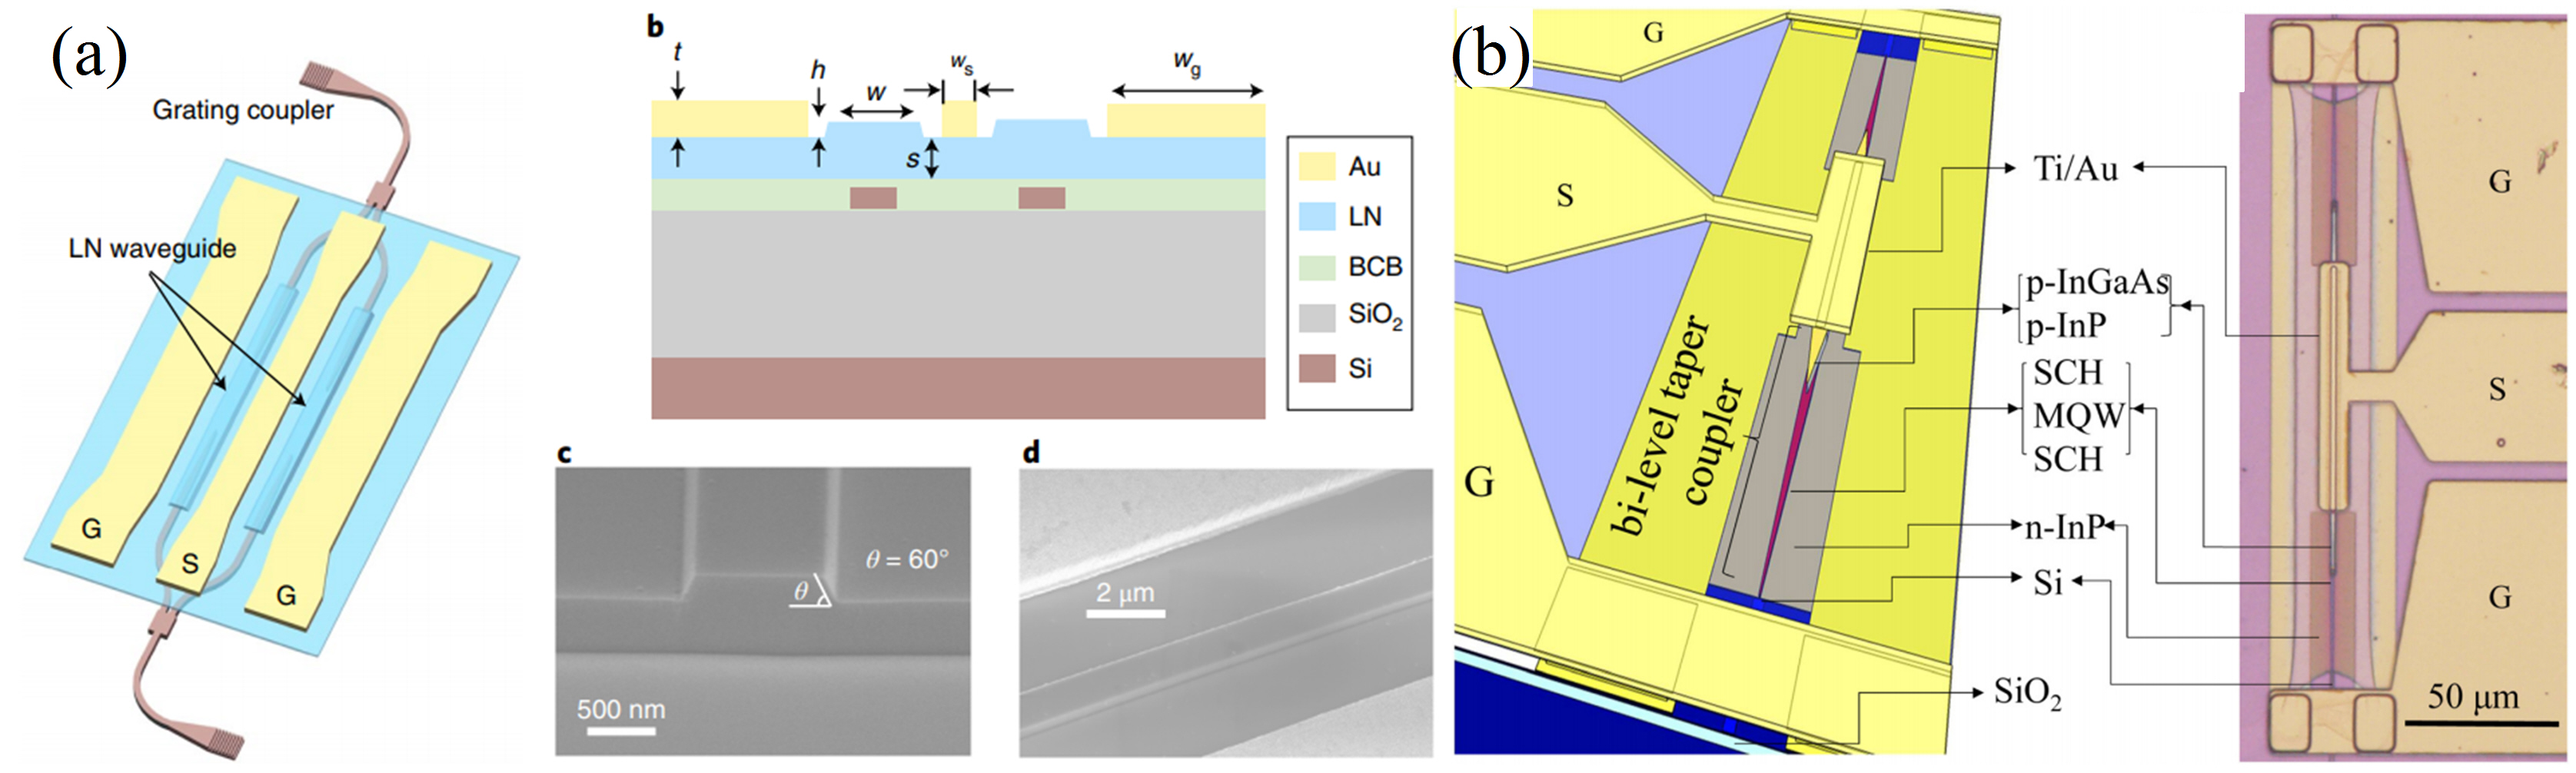
\includegraphics[width=16cm]{./Pictures/intro_external_modulator.jpg}
	\captionsetup{justification=centering}
	\caption{(a)马赫曾德调制器\cite{he2019high}(b)电吸收调制器\cite{huang2016low}}
	\label{intro_external_modulator}
\end{figure}


\subsection{气体检测领域的应用}

随着近几年来,我们对大气污染问题的越来越重视,各种污染物的检测成为政府进行科学合理地制定政策与规划的依据。相比于利用电化学传感器检测易受到干扰的问题,由于不同的气体分子的电子、振动、转动三个能级的不同,其都具有相应的光学吸收谱,故可以利用光学的方法来进行气体的特异性检测,其还具有非接触的特点。

图\ref{intro_ndir}所示为工业上基于NDIR(non-dispersion infrared absorption spectroscopy)的气体传感器示意图,可以实现CO和CO\SB{2}的浓度传感。该传感器从上端发射可以分别被CO和CO\SB{2}吸收的激光,利用CO和CO\SB{2}对不同的波长吸收不同,通过底部探测器得到的光强可以反推出气体的浓度。

\begin{figure}[htb]
	\centering
	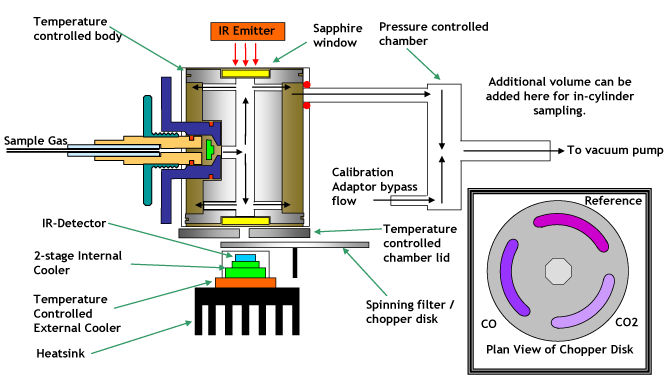
\includegraphics[width=14cm]{./Pictures/intro_ndir.png}
	\captionsetup{justification=centering}
	\caption{工业上基于NDIR的CO与CO\SB{2}传感器\cite{cambustionndir}}
	\label{intro_ndir}
\end{figure}

\section{论文的主要研究工作和创新点}
\subsection{主要内容}

本论文主要的研究工作基于对硅基混合集成自脉冲DFB激光器的研究以及其在三个领域的应用。第一个应用是在微波光子学领域,利用自脉冲DFB激光器的拍频效应,结合探测器可以生成频率可调的微波信号,实验还发现,该微波信号还可以通过注入外调制信号进行频率锁定。第二个应用是在光互联领域,利用光子共振现象,自脉冲DFB激光器可以提升直调带宽,实现更大的数据传输速率。第三个应用是在气体传感领域,利用自脉冲激光器双波长可调的特性,可以将一个激射波长设定到气体的吸收峰上,另一个激射波长位于吸收峰附近作为参考,通过比较,可以进行气体浓度的测量,为此,本文还设计了一个基于EDG的片上高分辨率光谱仪。本文还对在实际加工制作器件的过程中遇到的一些工艺问题做了相应的研究与改进。针对电子束曝光加工大尺寸器件的拼接错位问题,本文提出了一种叫做描边法的加工工艺;针对实验加工过程中刻蚀深度的控制,本文提出了一种根据颜色来判断SOI芯片刻蚀深度的方法,能够方便实验过程中刻蚀深度的确认。

本文的章节安排如下:

第一章为绪论,首先介绍了硅基光电子集成技术的发展背景,接着着重介绍了硅基光电子平台上的光源以及混合集成DFB激光器以及其在气体检测、微波光子学、光互联领域的应用。

第二章首先介绍了硅光集成器件设计中的基本理论和数值仿真方法。本文从麦克斯韦方程组出发,推导了光波导的模式特征方程,简要阐述了光波导模式理论,针对一般情况下波导中光场的传输问题,本文介绍了时域有限差分的数值计算方法。之后,本文介绍了DFB激光器的基本原理。最后,本文介绍了实验室加工制作硅基光子器件的基本方法。

第三章介绍了一种利用SOI芯片颜色来确定硅层厚度的方法,因为在实际器件制作过程中经常需要对SOI芯片做减薄工艺。本章首先介绍了薄硅在硅基光电子器件中的应用及其优势作为例子,然后介绍了光度学和色度学的一些基本内容,利用时域有限差分的数值计算方法,本文给出了不同硅层厚度下SOI芯片的反射谱,根据反射光谱得到了不同硅层厚度对应的颜色,发现当硅层厚度小于120~$nm$之后,随着硅层厚度的变化,颜色变化变得非常明显,这可以帮助实验人员快速确定硅层的厚度。本文将计算结果与实验进行了比较,取得了一致的结果。

第四章首先介绍了自脉冲DFB(distributed feedback laser)激光器及其原理,之后介绍了III-V族材料和硅的混合集成方法。本文设计并制作了一个硅基III-V混合集成的自脉冲DFB激光器,并测试了该自脉冲激光器的性能。产生的自脉冲可以用于微波光子学中光学微波信号的产生并发现了其频率锁定的现象。本文还发现了该自脉冲现象还可以用来提升激光器的调制带宽,并给出了相应的实验结果。

第五章首先结合上一章中自脉冲激光器有双波长的特性,设计了一套由激光器与光谱仪构成的气体浓度检测系统。之后介绍了片上光谱仪的几种实现方案,然后给出了基于EDG的硅基片上高分辨率光谱仪的设计,该光谱仪的输出波导采用密集阵列波导以提升光谱仪的分辨率。本文设计的光谱仪通道数为121,通道间隔为0.5~$nm$。受限于实验室的EBL加工条件,实验上,本文制作了只包含20通道的该EDG光谱仪作为方案的验证,实现了分辨率($\lambda/\Delta\lambda$)高达5571的实验结果,但是其通道间的串扰只有-4.3~dB。本文对实验结果进行了分析,给出了串扰的来源即其解决办法。

第六章对本文主要内容和各项工作进行总结,并展望了未来可以继续优化完善和深入探索的方向。

\subsection{本论文的主要创新点}
本文的创新点主要包括以下几个方面:

\begin{enumerate}[(1)]
	\item 
	本文首次得出了SOI芯片硅层厚度与其显示的颜色之间的关系,得益于硅的高折射率与在可见光波段处的吸收特性,我们可以得到非常丰富的颜色变化信息,尤其当硅层厚度小于120~$nm$时,几纳米的硅层厚度变化,就可以对应非常大的颜色变化,这可以用来快速且较准确地确定硅层的厚度。为了更方便的进行颜色比较,利用人眼对颜色差异的敏感特性,本文还专门开发了一款手机APP用于辅助确定硅层的厚度。根据实验显示,利用该软件,当硅层厚度小于120~$nm$时,可以达到较高的精度。
	\item 
	本文利用III-V族材料和硅的混合集成技术,制作了一个自脉冲DFB激光器。该自脉冲激光器的自脉冲效应可以用于产生光学微波信号,且该微波信号的带宽与激光器的线宽相关联,处于MHz量级。本文发现可以通过外加窄带微波信号,将自脉冲微波信号锁定到特定频率,且其线宽可以小于10~Hz,最小的锁定功率可以达到-17~dBm,为目前报道的最小值。该自脉冲激光器还可以利用光子共振现象提升激光器的调制带宽,本文给出了相应的实验结果,调制带宽可以达到23~GHz,实现了45~Gbps的数据传输速率。
	\item 
	本文提出了一套利用自脉冲激光器的双波长特性与光谱仪结合的气体浓度检测系统。其中一个波长位于气体的吸收峰上,另一个波长位于吸收峰旁作为参考。光谱仪采用基于EDG的设计,首次将密集波导阵列应用到EDG的输出波导中,使其输出波导之间的间距只有1~$\mu m$,提升了EDG光谱仪的分辨率。利用该设计可以在器件尺寸固定时提高光谱仪的分辨率或者在分辨率要求一定时,缩小器件的尺寸。该光谱仪采用双完美成像点的设计方法,包含121个通道,通道间隔0.5~$nm$,覆盖了在1550~$nm$波段60~$nm$的测量范围,并对边缘通道的性能进行了优化,使其通道均匀性更好。实验制作的器件尺寸为3~$mm~\times$~3~$mm$,通道数为20,通道间隔为0.5~$nm$,分辨率($\lambda/\Delta\lambda$)达到5571,是目前已知的基于片上EDG的光谱仪的最高值,且该EDG光谱仪具有集成121通道的潜力,这是其他设计方法较难实现的。
	\end{enumerate}

